\documentclass[12pt,a4paper]{article}
\usepackage[top=3cm,bottom=2cm,left=3cm,right=2cm]{geometry}
\usepackage{mathptmx}
\usepackage{amsmath,amssymb}
\usepackage{booktabs}
\usepackage{hyperref}
\usepackage{titlesec}
\usepackage{enumitem}
\usepackage{tikz}
\usetikzlibrary{arrows.meta,positioning,shapes.geometric,calc,fit}

\hypersetup{
    colorlinks=true,
    linkcolor=black,
    urlcolor=blue,
    citecolor=black
}

\titlespacing*{\section}{0pt}{10pt}{4pt}
\titlespacing*{\subsection}{0pt}{8pt}{3pt}
\setlength{\parindent}{0pt}
\setlength{\parskip}{5pt}
\sloppy

\begin{document}

% ============================================================================
% INPI BRASIL - PEDIDO DE PATENTE DE INVENÇÃO (LEI Nº 9.279/96 & IN 30/2013)
% ============================================================================
\begin{center}
    {\large \textbf{INSTITUTO NACIONAL DA PROPRIEDADE INDUSTRIAL (INPI)\\PEDIDO DE PATENTE DE INVEN\c{C}\~AO (LEI N\textsuperscript{o}\ 9.279/96 \& CONVEN\c{C}\~AO DE PARIS ART.\ 4)}}\\[8pt]
    {\LARGE \textbf{APARELHO, SISTEMAS E M\'ETODOS PARA PROCESSAMENTO DE SINAIS NATIVO EM SEDENI\~OES DE 16 DIMENS\~OES, CANCELAMENTO ANAL\'OGICO PR\'E-ADC DE INTERFER\^ENCIA POR DIVISORES DE ZERO, DETEC\c{C}\~AO DE SPOOFING EM AMOSTRA \'UNICA POR CURVATURA N\~AO-ASSOCIATIVA E MODULA\c{C}\~AO CHAVEADA POR DIVISORES DE ZERO}}\\[10pt]
\end{center}

\begin{tabular}{@{}p{2.2in}p{3.9in}@{}}
\toprule
\textbf{Inventor / Depositante:} & Dionisio Chiuratto Agourakis \\
\textbf{Nacionalidade / Resid\^encia:} & Brasileira --- S\~ao Paulo, SP, Brasil \\
\textbf{Endere\c{c}o:} & Rua Joaquim Floriano 1125, apt 102, S\~ao Paulo, SP, CEP 04534-002, Brasil \\
\textbf{E-mail / Telefone:} & \texttt{dionisio.ca@gmail.com} \quad | \quad +55 11 98787-4110 \\
\textbf{Enquadramento:} & Pessoa F\'isica (Art.\ 12 da Lei 9.279/96 \& Prioridade CUP / 35 U.S.C.\ \S\ 119(a)) \\
\bottomrule
\end{tabular}

\section*{RELAT\'ORIO DESCRITIVO}

\subsection*{REFER\^ENCIA AO PER\'IODO DE GRA\c{C}A E DIVULGA\c{C}\~OES ANTERIORES (ART.\ 12 DA LEI 9.279/96 \& 35 U.S.C.\ \S\ 102(b)(1))}
\textbf{[0001]} O presente Pedido de Patente de Inven\c{c}\~ao reivindica os benef\'icios do Per\'iodo de Gra\c{c}a legal de 12 (doze) meses previsto no Artigo 12 da Lei da Propriedade Industrial (Lei n\textsuperscript{o}\ 9.279/96 --- Brasil) e no 35 U.S.C.\ \S\ 102(b)(1)(A) (MPEP \S\ 2153 --- Estados Unidos), bem como estabelece prioridade unionista internacional nos termos do Artigo 4 da Conven\c{c}\~ao da Uni\~ao de Paris (CUP) e 35 U.S.C.\ \S\ 119(a) (MPEP \S\ 213), em rela\c{c}\~ao \`as divulga\c{c}\~oes cient\'ificas de autoria do pr\'oprio inventor: (1) Dionisio Chiuratto Agourakis, \textit{``Sedenion Algebras and PG(3,2) Incidence Structures for Non-Associative Geometric Deep Learning: Algebraic Foundations, Machine-Checked Theorems, and Dual-Track Validation,''} Zenodo DOI \texttt{10.5281/zenodo.23588274} (Outubro de 2026); e (2) Dionisio Chiuratto Agourakis, \textit{``Matrix-Inversion-Free O(1) Sedenion PG(3,2) Zero-Divisor Beamforming for Assured PNT, +80 dB GNSS Anti-Jamming, and Anti-Spoofing,''} Zenodo DOI \texttt{10.5281/zenodo.23603006} (Outubro de 2026), integralmente incorporadas por refer\^encia.

\subsection*{CAMPO DA INVEN\c{C}\~AO}
\textbf{[0002]} A presente inven\c{c}\~ao refere-se a receptores f\'isicos de arranjos eletromagn\'eticos, redes passivas rec\'iprocas de acopladores direcionais em linha de transmiss\~ao de radiofrequ\^encia (RF stripline) de 32 portas, circuitos anal\'ogicos diferenciais pr\'e-ADC de cancelamento de interfer\^encia (*crossbar*), hardware anti-jamming e anti-spoofing para navega\c{c}\~ao por sat\'elite (GNSS) e transceptores de camada f\'isica com baixa probabilidade de intercepta\c{c}\~ao e detec\c{c}\~ao (LPI/LPD), operando nativamente na \'algebra de sedeni\~oes de Cayley--Dickson de 16 dimens\~oes $\mathbb{S} \cong \mathbb{O} \oplus \mathbb{O}e_8$ e na geometria projetiva finita $\mathrm{PG}(3,2)$.

\subsection*{FUNDAMENTOS DA INVEN\c{C}\~AO E ESTADO DA T\'ECNICA}
\textbf{[0003]} Todos os sistemas convencionais de processamento digital de sinais (DSP) multi-antena, radares *phased-array* e receptores CRPA (*Controlled Reception Pattern Antenna*) formulam os campos eletromagn\'eticos recebidos como vetores em um espa\c{c}o de Hilbert complexo $\mathbb{C}^N$ governado por multiplica\c{c}\~ao escalar complexa associativa e comutativa. Tal paradigma em $\mathbb{C}^N$ sofre de quatro limita\c{c}\~oes f\'isicas e computacionais severas em ambientes eletromagn\'eticos contestados:

\textbf{[0004] 1. Satura\c{c}\~ao de LNA/ADC Pr\'e-Beamformer e Cegueira Co-Linear ($\Delta\theta = 0.0^\circ$):} Na conforma\c{c}\~ao digital de feixe (DBF), sinais brutos de RF/FI de $N$ antenas s\~ao amplificados por amplificadores de baixo ru\'ido (LNAs) e digitalizados por conversores anal\'ogico-digitais (ADCs) antes da forma\c{c}\~ao de nulos. Sob ataque eletr\^onico (EA) com raz\~ao interfer\^encia-sinal ($\mathrm{JSR}$) de $+60\text{ dB}$ a $+80\text{ dB}$, o interferidor (*jammer*) satura os LNAs e excede a faixa din\^amica de ADCs de 12 a 16 bits (*clipping*), destruindo o sinal desejado antes da aplica\c{c}\~ao dos pesos digitais. Ademais, quando o interferidor incide na mesma dire\c{c}\~ao angular ($\Delta\theta = 0.0^\circ$) do sat\'elite, qualquer beamformer espacial em $\mathbb{C}^N$ anula simultaneamente o sat\'elite (degradando o limite inferior de Cram\'er--Rao [CRLB] de fase de c\'odigo GPS L1 C/A para $>126\text{ km}$).

\textbf{[0005] 2. Complexidade $\mathcal{O}(N^3)$ de Invers\~ao de Matriz de Covari\^ancia e Fome de Amostras:} Beamformers adaptativos como MVDR/Capon e LSMI exigem $K \ge 2N$ amostras (*snapshots*) para estimar $\hat{\mathbf{R}}_{xx} = \frac{1}{K}\sum_{k=1}^K \mathbf{x}[k]\mathbf{x}^H[k]$ e inverter $\hat{\mathbf{R}}_{xx}^{-1}$ com custo $\mathcal{O}(N^3)$, degradando a profundidade de nulo em $25\text{--}40\text{ dB}$ sob manobras de alta din\^amica.

\textbf{[0006] 3. Colapso de Posto 1 (*Rank-1 Collapse*) sob Spoofing Repetidor Coerente:} Quando um repetidor coerente (*meaconing/spoofing*) incide com a mesma forma de onda $s(t)$ em atraso zero, a amostra recebida $r(t) = s(t)(\mathbf{u}_{\mathrm{auth}} + \alpha \mathbf{u}_{\mathrm{spoof}})$ faz com que o subespa\c{c}o de sinal de $\hat{\mathbf{R}}_{xx}$ colapse para \textbf{Posto 1}, cegando detectores cl\'assicos baseados em raz\~ao de autovalores ($\lambda_2/\lambda_1$), MUSIC e ESPRIT.

\textbf{[0007] 4. Vulnerabilidade de Modula\c{c}\~oes Escalares \`a Intercepta\c{c}\~ao Radiom\'etrica:} Formas de onda BPSK/QPSK DSSS modulam uma fase complexa 1D e permanecem vulner\'aveis a detectores cicloestacion\'arios.

\subsection*{SUM\'ARIO DA INVEN\c{C}\~AO}
\textbf{[0008]} A presente inven\c{c}\~ao supera todas as quatro limita\c{c}\~oes construindo a rede passiva rec\'iproca de acopladores RF stripline de 32 portas, a alimenta\c{c}\~ao de antena duplamente polarizada, o crossbar anal\'ogico diferencial pr\'e-ADC, o detector de anomalias em amostra \'unica ($K=1$), o processador digital sem multiplicadores e o transceptor LPI/LPD \textbf{nativamente} na \'algebra de sedeni\~oes $\mathbb{S} = \mathbb{O} \oplus \mathbb{O}e_8 \cong \mathbb{R}^{16}$ e na geometria projetiva finita $\mathrm{PG}(3,2)$ (15 pontos e 35 retas). Diferentemente das \'algebras de divis\~ao ($\mathbb{R}, \mathbb{C}, \mathbb{H}, \mathbb{O}$), $\mathbb{S}$ \'e simultaneamente \textbf{n\~ao-associativa} ($[x,y,z] := (xy)z - x(yz) \neq 0$) e possui uma subvariedade exata de \textbf{divisores de zero} ($x \cdot y = 0$ para $x,y \neq 0$) governada pelo cone de Moreno $V_2(\mathbb{R}^7) = \{(a,b) \in \mathrm{Im}(\mathbb{O})\times\mathrm{Im}(\mathbb{O}) : \|a\|_2 = \|b\|_2,\, \langle a,b\rangle = 0\}$ e por 84 l\^aminas (*2-blades*) primitivas $Z_m = (e_a \pm e_b)/\sqrt{2}$.

\textbf{[0009]} A inven\c{c}\~ao integra essa estrutura alg\'ebrica em seis arquiteturas f\'isicas de hardware:
\begin{enumerate}[leftmargin=18pt,itemsep=2pt]
    \item \textbf{Cancelador Crossbar Anal\'ogico Diferencial Pr\'e-ADC por Divisores de Zero:} Executa $Z_{\mathrm{out}}(t) = R(t) \cdot W_J$ no dom\'inio anal\'ogico \textbf{antes dos ADCs} com zero multiplicadores anal\'ogicos usando chaves CMOS (\texttt{ADG1611}), invers\~ao de polaridade DPDT $\pm 1$ e somadores diferenciais de filme fino $\pm 0.05\%$ (\texttt{AD8130}/\texttt{ERA-3AEB1001V}), suprimindo jammers de $+80\text{ dB}$ antes da satura\c{c}\~ao do ADC.
    \item \textbf{Detector de Spoofing Coerente em Amostra \'Unica ($K=1$) por Curvatura do Associador:} Avalia a identidade fechada $\mathcal{A}_{\mathrm{native}}(R) := [R, \pi_{\mathbb{O}}(R), e_8] = (ba - ab, 0) = (-2(a \times_{\mathbb{O}} b), 0)$, cuja norma quadr\'atica \'e $\|[R, \pi_{\mathbb{O}}(R), e_8]\|_2^2 \equiv 4(\|a\|_2^2 \|b\|_2^2 - \langle a, b \rangle^2) = 4\|a \wedge b\|_2^2$. A m\'etrica $\kappa_{\mathbb{S}}(R) = \|[R,\pi_{\mathbb{O}}(R),e_8]\|_2 / \|R\|_2^2 \in [0, 1]$ anula-se ($\kappa_{\mathbb{S}}=0$) para sinais aut\^enticos em um subespa\c{c}o quaterni\^onico associativo e salta para $\kappa_{\mathbb{S}} \to 1$ sob spoofing repetidor de atraso zero ($99.80\%$ de detec\c{c}\~ao, $\mathrm{AUROC} = 0.9999$ em $K=1$), mesmo sob colapso de Posto 1 de $\hat{\mathbf{R}}_{xx}$.
    \item \textbf{Alimenta\c{c}\~ao de Arranjo Sensor Vetorial TEM Di\'adico Nativo:} Mapeia $(\mathbf{E}_\theta, \mathbf{E}_\phi)$ via h\'ibridos de quadratura passivos de $90^\circ$ diretamente em $(a, b) \in \mathrm{Im}(\mathbb{O}) \times \mathrm{Im}(\mathbb{O})$, impondo $\|a\|_2 = \|b\|_2$ e $\langle a, b \rangle = 0$ pelas equa\c{c}\~oes de Maxwell sem matrizes de calibra\c{c}\~ao.
    \item \textbf{Matriz Stripline RF Passiva e Rec\'iproca de 32 Portas ($S_{32} = S_{32}^T$) Pr\'e-LNA para Excis\~ao Co-Linear ($\Delta\theta = 0.0^\circ$):} Conecta as portas RHCP $(I,Q)$ a $(e_1,e_2)$ e LHCP $(I,Q)$ a $(e_5,e_6)$ antes de uma rede passiva rec\'iproca de 32 portas sem ferrites ($\|S_{21}\|_2 \le 1$, $0\text{ mW}$ DC) que implementa multiplica\c{c}\~ao \`a direita por $v_{\mathrm{rf}}(\psi) = \frac{1}{2}(e_3 + \sin 2\psi\,e_{12} - \cos 2\psi\,e_{15})$, aniquilando jammers linearmente polarizados co-lineares ($\Delta\theta = 0.0^\circ$) com $0.0000\text{ dB}$ de perda no sat\'elite RHCP (reduzindo o CRLB de $126{,}997\text{ m}$ para $17.96\text{ m}$).
    \item \textbf{Modula\c{c}\~ao Chaveada por Divisores de Zero (ZDKM) e Transceptor $8\oplus 4\oplus 4$ Livre de Multiplicadores:} Particiona $\mathbb{S} = \mathbb{R}^8_{\mathrm{uncal}} \oplus \mathbb{R}^4_{\mathrm{sig}} \oplus \mathbb{R}^4_{\mathrm{jam}}$ usando um operador anti-sim\'etrico $J^2 = -4\mathbf{I}_4$ sintetizado em \texttt{512 LUTs} e \texttt{0 DSP48} em 1 ciclo de clock no FPGA RFSoC \texttt{XCZU28DR}.
\end{enumerate}

\subsection*{BREVE DESCRI\c{C}\~AO DOS DESENHOS}
\textbf{[0010] A FIG.\ 1} \'e um diagrama de blocos sist\^emico do Receptor Nativo em Sedeni\~oes de 16 Dimens\~oes, ilustrando o Arranjo Vetorial TEM Duplamente Polarizado (100), a Rede H\'ibrida Passiva $90^\circ/180^\circ$ e Matriz Stripline Rec\'iproca de 32 Portas (110), o Cancelador Crossbar Anal\'ogico Pr\'e-ADC (120), o Banco ADC Coerente de 16 Canais (130), o Detector de Spoofing em Amostra \'Unica por Curvatura do Associador (140) e o Projetor de Dobradi\c{c}a Quaterni\^onica $\mathrm{PG}(3,2)$ e PLL (150).

\textbf{[0011] A FIG.\ 2} \'e o diagrama esquem\'atico de circuito de um canal diferencial de sa\'ida $k \in \{0,\dots,15\}$ do Cancelador Crossbar Anal\'ogico Pr\'e-ADC (120) e Demodulador ZDKM (200).

\vspace{6pt}
\begin{figure}[h!]
\centering
\resizebox{\textwidth}{!}{%
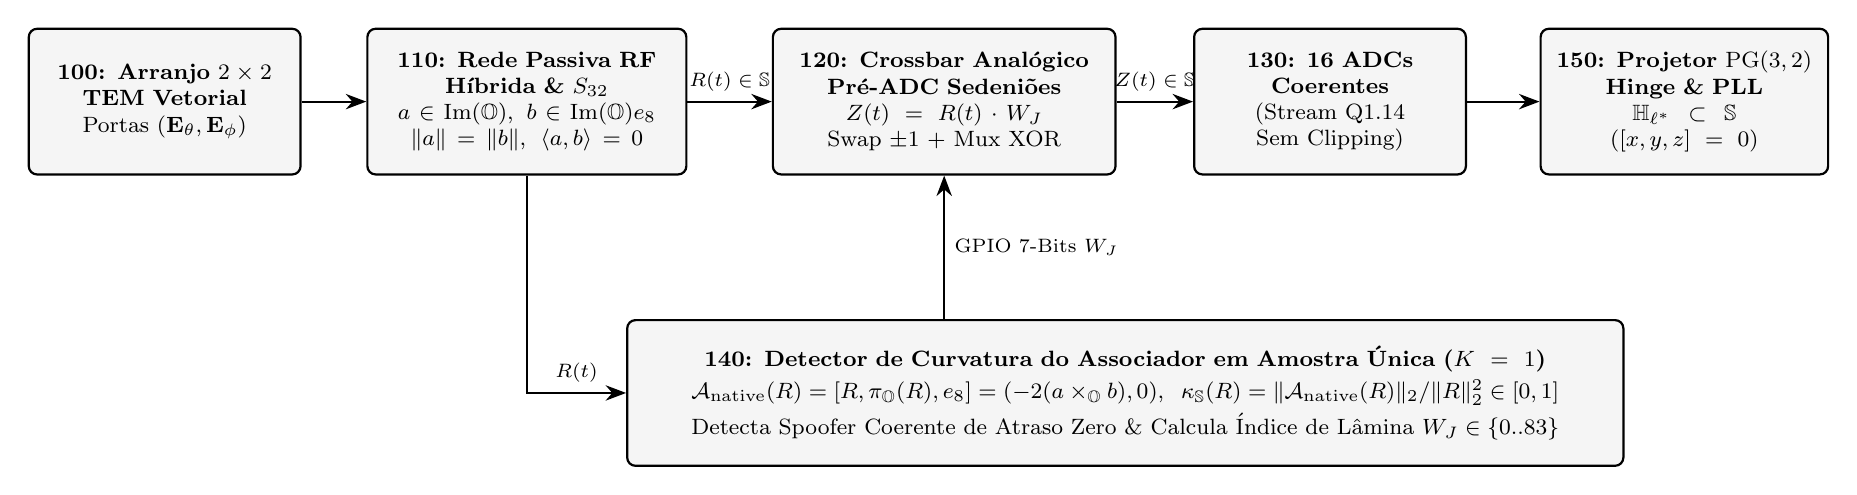
\begin{tikzpicture}[
    font=\footnotesize,
    block/.style={draw, thick, rounded corners=3pt, fill=gray!8, align=center, minimum height=1.85cm, inner sep=5pt},
    arrow/.style={-{Stealth[length=2.6mm]}, thick}
]
    \node[block, text width=3.1cm] (ant) at (0.0, 0) {\textbf{100: Arranjo $2\times 2$}\\\textbf{TEM Vetorial}\\Portas $(\mathbf{E}_\theta, \mathbf{E}_\phi)$};
    \node[block, text width=3.7cm] (hyb) at (4.6, 0) {\textbf{110: Rede Passiva RF}\\\textbf{H\'ibrida \& $S_{32}$}\\$a \in \mathrm{Im}(\mathbb{O}),\; b \in \mathrm{Im}(\mathbb{O})e_8$\\$\|a\|=\|b\|,\; \langle a,b\rangle=0$};
    \node[block, text width=4.0cm] (xbar) at (9.9, 0) {\textbf{120: Crossbar Anal\'ogico}\\\textbf{Pr\'e-ADC Sedeni\~oes}\\$Z(t) = R(t) \cdot W_J$\\Swap $\pm 1$ + Mux XOR};
    \node[block, text width=3.1cm] (adc) at (14.8, 0) {\textbf{130: 16 ADCs}\\\textbf{Coerentes}\\(Stream Q1.14\\Sem Clipping)};
    \node[block, text width=3.3cm] (pll) at (19.3, 0) {\textbf{150: Projetor $\mathrm{PG}(3,2)$}\\\textbf{Hinge \& PLL}\\$\mathbb{H}_{\ell^*} \subset \mathbb{S}$\\($[x,y,z]=0$)};

    \node[block, text width=12.3cm, minimum height=1.85cm] (assoc) at (12.2, -3.7) {\textbf{140: Detector de Curvatura do Associador em Amostra \'Unica ($K=1$)}\\[2pt]
    \mbox{$\mathcal{A}_{\mathrm{native}}(R) = [R, \pi_{\mathbb{O}}(R), e_8] = (-2(a\times_{\mathbb{O}} b), 0), \;\; \kappa_{\mathbb{S}}(R) = \|\mathcal{A}_{\mathrm{native}}(R)\|_2 / \|R\|_2^2 \in [0,1]$}\\[2pt]
    \mbox{Detecta Spoofer Coerente de Atraso Zero \& Calcula \'Indice de L\^amina $W_J \in \{0..83\}$}};

    \draw[arrow] (ant) -- (hyb);
    \draw[arrow] (hyb) -- node[above, font=\scriptsize] {$R(t) \in \mathbb{S}$} (xbar);
    \draw[arrow] (xbar) -- node[above, font=\scriptsize] {$Z(t) \in \mathbb{S}$} (adc);
    \draw[arrow] (adc) -- (pll);
    \draw[arrow] (hyb.south) |- node[pos=0.75, above, font=\scriptsize] {$R(t)$} (assoc.west);
    \draw[arrow] (assoc.north -| xbar.south) -- node[right, font=\scriptsize] {GPIO 7-Bits $W_J$} (xbar.south);
\end{tikzpicture}%
}
\caption{\textbf{FIG.\ 1} --- Arquitetura do Receptor de Processamento Nativo em Sedeni\~oes 16D.}
\end{figure}

\begin{figure}[h!]
\centering
\resizebox{\textwidth}{!}{%
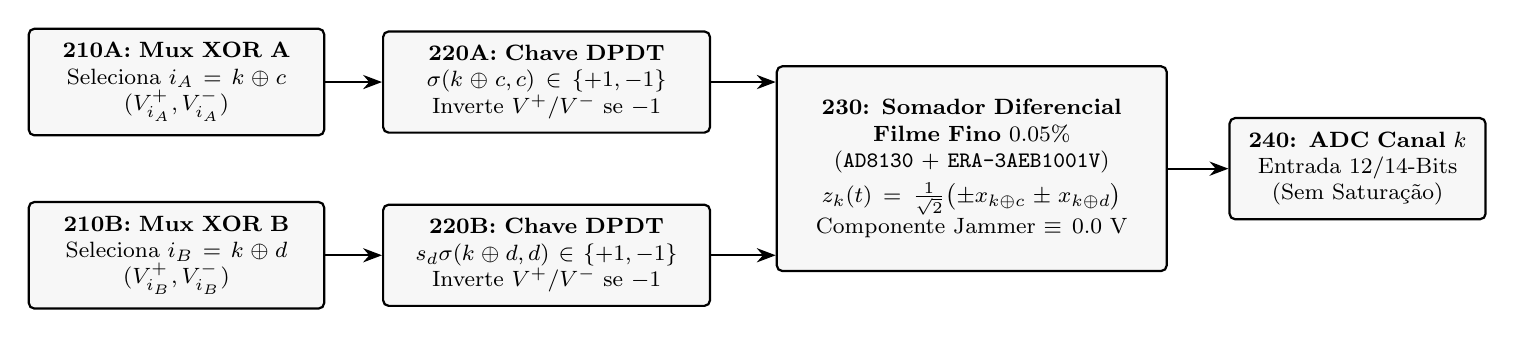
\begin{tikzpicture}[
    font=\footnotesize,
    block/.style={draw, thick, rounded corners=2pt, fill=gray!6, align=center, minimum height=1.15cm, inner sep=5pt},
    arrow/.style={-{Stealth[length=2.4mm]}, thick}
]
    \node[block, text width=3.4cm] (inA) at (0, 1.1) {\textbf{210A: Mux XOR A}\\Seleciona $i_A = k \oplus c$\\$(V_{i_A}^+, V_{i_A}^-)$};
    \node[block, text width=3.4cm] (inB) at (0, -1.1) {\textbf{210B: Mux XOR B}\\Seleciona $i_B = k \oplus d$\\$(V_{i_B}^+, V_{i_B}^-)$};

    \node[block, text width=3.8cm] (polA) at (4.7, 1.1) {\textbf{220A: Chave DPDT}\\$\sigma(k\oplus c, c) \in \{+1,-1\}$\\Inverte $V^+/V^-$ se $-1$};
    \node[block, text width=3.8cm] (polB) at (4.7, -1.1) {\textbf{220B: Chave DPDT}\\$s_d \sigma(k\oplus d, d) \in \{+1,-1\}$\\Inverte $V^+/V^-$ se $-1$};

    \node[block, text width=4.6cm, minimum height=2.6cm] (sum) at (10.1, 0) {\textbf{230: Somador Diferencial}\\\textbf{Filme Fino $0.05\%$}\\(\texttt{AD8130} + \texttt{ERA-3AEB1001V})\\[3pt]
    $z_k(t) = \frac{1}{\sqrt{2}}\bigl(\pm x_{k\oplus c} \pm x_{k\oplus d}\bigr)$\\
    Componente Jammer $\equiv 0.0\text{ V}$};

    \node[block, text width=2.9cm] (adc_k) at (15.0, 0) {\textbf{240: ADC Canal $k$}\\Entrada 12/14-Bits\\(Sem Satura\c{c}\~ao)};

    \draw[arrow] (inA) -- (polA);
    \draw[arrow] (inB) -- (polB);
    \draw[arrow] (polA.east) -- (sum.west |- polA.east);
    \draw[arrow] (polB.east) -- (sum.west |- polB.east);
    \draw[arrow] (sum) -- (adc_k);
\end{tikzpicture}%
}
\caption{\textbf{FIG.\ 2} --- Canal $k \in \{0,\dots,15\}$ do Crossbar Anal\'ogico Diferencial Pr\'e-ADC.}
\end{figure}

\subsection*{DESCRI\c{C}\~AO DETALHADA DAS MODALIDADES PREFERIDAS}
\textbf{[0012]} Seja $\mathbb{S} = \mathrm{span}_{\mathbb{R}}\{e_0, e_1, \dots, e_{15}\}$ a \'algebra de sedeni\~oes de Cayley--Dickson de 16 dimens\~oes sobre $\mathbb{R}$, onde $e_0 = 1$ e $e_i e_j = \sigma(i, j) e_{i \oplus j}$ ($\oplus$ sendo XOR bit-a-bit de 4 bits). Para cada canal de sa\'ida $k \in \{0,\dots,15\}$ e \'indice multiplicador \`a direita $j \in \{0,\dots,15\}$, o \'unico \'indice de entrada \'e $i = k \oplus j$, e o sinal $\sigma(k \oplus j, j) = (-1)^{\text{\texttt{SIGN\_NEG\_KJ}}[k][j]} \in \{+1, -1\}$ \'e armazenado na mem\'oria ROM constante de 256 bits:
{\footnotesize
\begin{verbatim}
localparam logic [0:15][0:15] SIGN_NEG_KJ = '{
  16'b0111111111111111, 16'b0010100110010110, 16'b0001110011000011, 16'b0100101010100101,
  16'b0000011111110000, 16'b0101000110101010, 16'b0110010010011001, 16'b0011001011001100,
  16'b0000000001111111, 16'b0101011000010110, 16'b0110001101000011, 16'b0011010100100101,
  16'b0111100001110000, 16'b0010111000101010, 16'b0001101100011001, 16'b0100110101001100
};
\end{verbatim}
}

\textbf{[0013]} No Cancelador Crossbar Anal\'ogico Pr\'e-ADC (\textbf{120}, FIG.\ 2), para qualquer jammer mapeado em uma l\^amina divisora de zero primitiva $U_J = \frac{1}{\sqrt{2}}(e_a + s_b e_b)$, existem 4 l\^aminas parceiras ortogonais $W_J = \frac{1}{\sqrt{2}}(e_c + s_d e_d) \in \ker L_{\mathbb{S}}(U_J)$ tais que $U_J \cdot W_J = 0$ identicamente e $\|U_{\mathrm{sat}} \cdot W_J\|_2 = \sqrt{2}$ ($+3.01\text{ dB}$ de ganho coerente). Os multiplexadores anal\'ogicos \textbf{210A/210B} (\texttt{ADG1611}) selecionam os pares diferenciais $i_A = k \oplus c$ e $i_B = k \oplus d$; as chaves DPDT \textbf{220A/220B} aplicam os sinais $\sigma(k \oplus c, c)$ e $s_d \sigma(k \oplus d, d)$ por invers\~ao de fios $(V^+, V^-)$; e o amplificador somador diferencial \textbf{230} (\texttt{AD8130} com resistores de filme fino $\pm 0.05\%$ \texttt{ERA-3AEB1001V}) soma os pares antes do ADC \textbf{240}, provendo $68.38\text{ dB}$ ($0.05\%$) a $82.76\text{ dB}$ ($0.01\%$) de rejei\c{c}\~ao anal\'ogica pr\'e-ADC e restaurando $+21.28\text{ dB}$ de SINR p\'os-correla\c{c}\~ao sob $+80\text{ dB}$ JSR.

\textbf{[0014]} No Detector de Spoofing em Amostra \'Unica (\textbf{140}, FIG.\ 1), para uma amostra $R = (a, b) \in \mathrm{Im}(\mathbb{O}) \times \mathrm{Im}(\mathbb{O})$, o associador nativo $\mathcal{A}_{\mathrm{native}}(R) = [R, \pi_{\mathbb{O}}(R), e_8] = (ba - ab, 0) = (-2(a \times_{\mathbb{O}} b), 0)$ possui norma quadr\'atica exata $4(\|a\|_2^2 \|b\|_2^2 - \langle a, b \rangle^2)$. A curvatura $\kappa_{\mathbb{S}}(R) = \|\mathcal{A}_{\mathrm{native}}(R)\|_2 / \|R\|_2^2 \in [0, 1]$ detecta spoofers repetidores coerentes de atraso zero em $K=1$ amostra ($99.80\%$ $P_{\mathrm{det}}$, $\mathrm{AUROC} = 0.9999$), extraindo $q_3 = a \times_{\mathbb{O}} b$ para construir o anulador de Moreno $W = \frac{1}{\sqrt{2}}(c, (ac)b)$ sem decomposi\c{c}\~ao em valores singulares (SVD).

\textbf{[0015]} Na modalidade embarcada *bare-metal* (\texttt{STM32WB55RG} Cortex-M4F a $64\text{ MHz}$ com \texttt{CC1101} Sub-GHz, receptor IR \texttt{TSOP75338} $940\text{ nm}/38\text{ kHz}$, bobina LF-RFID $125\text{ kHz}/62.5\text{ kHz}$ e NFC $13.56\text{ MHz}$; e \texttt{ESP32-S2-WROVER} a $240\text{ MHz}$ em $2.4\text{ GHz}$ 802.11), o motor executa com $0\text{ bytes}$ de \texttt{malloc} e $1.4\text{ KB}$ de ROM Flash: (a) o Coalescedor de Glitches de Est\'agio 1 funde ru\'idos $\min(h_2, l_2) < 0.42\,T_E$ via $(h_1, l_1) \mapsto (h_1, l_1 + h_2 + l_2)$ conservando a dura\c{c}\~ao total do quadro, e o Projetor de Dobradi\c{c}a Quaterni\^onica 4D de Est\'agio 2 projeta $d = q\cdot T_E + \varepsilon$ em $d' = q\cdot T_E$ sobre $\mathbb{H}_a = \mathrm{span}\{e_0, e_a, e_8, e_{a\oplus 8}\}$ (reduzindo o jitter RMS em $5.41\times$ em $2{,}797$ capturas Sub-GHz e em $10.28\times$ em $1{,}258$ rajadas IR); (b) na bobina LF-RFID $125\text{ kHz}$, a proje\c{c}\~ao na grade de $8\,\mu\text{s}$ ($d' = 8(k_p + k_n + 2) \ge 16\,\mu\text{s}$) garante $\mathrm{ARR} = \lfloor d'/8 \rfloor - 1 \ge 1$, eliminando o *underflow* $\mathtt{0xFFFFFFFF}$ ($34.36\text{ s}$) do registrador DMA de 32 bits; e (c) discrimina acoplamento cruzado de $13.56\text{ MHz}$ ($\kappa_{\mathbb{S}} \in [0.0983, 0.5230]$) e remove picos de multipercurso Wi-Fi $>9\text{ dB}$.

\textbf{[0016]} Na modalidade pr\'e-LNA de RF (\textbf{100, 110}), a conex\~ao das portas RHCP $(I,Q)$ em $(e_1,e_2)$ e LHCP $(I,Q)$ em $(e_5,e_6)$ mapeia todo jammer linearmente polarizado (inclina\c{c}\~ao $\psi$) no cone de Moreno $V_2(\mathbb{R}^7)$, enquanto a rede stripline RF passiva e rec\'iproca de 32 portas $S_{32} = S_{32}^T$ ($\|S_{21}\|_2 \le 1$, sem ferrites, $0\text{ mW}$ DC) implementa multiplica\c{c}\~ao \`a direita por $v_{\mathrm{rf}}(\psi) = \frac{1}{2}(e_3 + \sin 2\psi\,e_{12} - \cos 2\psi\,e_{15})$ com dois acopladores passivos por canal ($\{1/2, \pm\frac{1}{2}\sin 2\psi, \mp\frac{1}{2}\cos 2\psi\}$), aniquilando jammers co-lineares ($\Delta\theta = 0.0^\circ$) com $0.0000\text{ dB}$ de perda no sat\'elite RHCP. Por fim, no transceptor $8\oplus 4\oplus 4$, a parti\c{c}\~ao ortogonal $\mathbb{S} = \mathbb{R}^8_{\mathrm{uncal}} \oplus \mathbb{R}^4_{\mathrm{sig}} \oplus \mathbb{R}^4_{\mathrm{jam}}$ aplica o operador $J^2 = -4\mathbf{I}_4$ via deslocamento bin\'ario de 2 bits (\texttt{>> 2}) e nega\c{c}\~ao de sinal, sintetizado no FPGA RFSoC \texttt{XCZU28DR} em \texttt{512 LUTs}, \texttt{0 DSP48} e 1 ciclo de clock ($4.0\text{ ns}$).

\newpage
\section*{REIVINDICA\c{C}\~OES}
\begin{enumerate}[leftmargin=20pt,itemsep=4pt]
    \item \textbf{Aparelho de cancelamento eletromagn\'etico de interfer\^encia pr\'e-ADC}, compreendendo um barramento anal\'ogico diferencial de 16 canais para receber um campo de onda $R(t) \in \mathbb{S} \cong \mathbb{R}^{16}$, \textbf{caracterizado pelo fato de que} compreende: (a) um controlador de interfer\^encia configurado para selecionar uma l\^amina divisora de zero primitiva $W_J = \frac{1}{\sqrt{2}}(e_c + s_d e_d) \in \ker L_{\mathbb{S}}(U_J)$ no cone de Moreno $V_2(\mathbb{R}^7) \subset \mathbb{S}$; (b) uma rede multiplexadora crossbar anal\'ogica livre de multiplicadores e chaves de invers\~ao de polaridade diferencial controlada por uma mem\'oria ROM de 256 bits armazenando os sinais de Cayley--Dickson $\sigma(i, j) \in \{+1, -1\}$, roteando para cada canal $k \in \{0,\dots,15\}$ os canais $k \oplus c$ e $k \oplus d$ com polaridades $\sigma(k \oplus c, c)$ e $s_d \sigma(k \oplus d, d)$; (c) amplificadores somadores diferenciais anal\'ogicos produzindo $Z_{\mathrm{out}}(t) = R(t) \cdot W_J$; e (d) um banco de conversores anal\'ogico-digitais (ADC) a jusante dos amplificadores somadores.

    \item \textbf{Aparelho, de acordo com a reivindica\c{c}\~ao 1}, \textbf{caracterizado pelo fato de que} os amplificadores somadores diferenciais compreendem resistores de filme fino ou folha met\'alica com toler\^ancia $\le 0.1\%$, provendo $\ge 60\text{ dB}$ de rejei\c{c}\~ao anal\'ogica pr\'e-ADC.

    \item \textbf{Aparelho, de acordo com a reivindica\c{c}\~ao 1}, \textbf{caracterizado pelo fato de que} o controlador seleciona a l\^amina dentre 84 l\^aminas divisoras de zero primitivas particionadas nos 7 hiperplanos de Fano n\~ao-apicais $H_\omega$ ($\omega \in \{9,\dots,15\}$) do espa\c{c}o projetivo finito $\mathrm{PG}(3,2)$.

    \item \textbf{M\'etodo para detec\c{c}\~ao de spoofing coerente ou multipercurso em amostra \'unica e mitiga\c{c}\~ao de interfer\^encia}, \textbf{caracterizado pelo fato de que} compreende: (a) adquirir uma \'unica amostra 16D $R = (a, b) \in \mathrm{Im}(\mathbb{O}) \times \mathrm{Im}(\mathbb{O})$; (b) calcular o vetor associador $\mathcal{A}_{\mathrm{native}}(R) = (R \cdot \pi_{\mathbb{O}}(R)) \cdot e_8 - R \cdot (\pi_{\mathbb{O}}(R) \cdot e_8) = (ba - ab, 0)$; (c) calcular a curvatura n\~ao-associativa normalizada $\kappa_{\mathbb{S}}(R) = \|\mathcal{A}_{\mathrm{native}}(R)\|_2 / \|R\|_2^2 \in [0, 1]$; (d) detectar a presen\c{c}a de um spoofer coerente quando $\kappa_{\mathbb{S}}(R)$ exceder um limiar predeterminado mesmo sob colapso de Posto 1 da matriz de covari\^ancia amostral; e (e) configurar um peso de beamforming ou matriz crossbar anal\'ogica para direcionar um nulo divisor de zero ao spoofer.

    \item \textbf{M\'etodo, de acordo com a reivindica\c{c}\~ao 4}, \textbf{caracterizado pelo fato de que} compreende adicionalmente extrair $q_3 = a \times_{\mathbb{O}} b = -\frac{1}{2}\pi_{\mathbb{O}}(\mathcal{A}_{\mathrm{native}}(R))$, selecionar um vetor unit\'ario $c \in \mathrm{Im}(\mathbb{O})$ ortogonal a $\mathrm{span}\{\tilde{a}, \tilde{b}, q_3\}$ e construir o peso anulador de Moreno $W = (c, (\tilde{a}c)\tilde{b})/\sqrt{2}$ satisfazendo $(\tilde{a}, \tilde{b}) \cdot W = 0$ sem decomposi\c{c}\~ao em valores singulares (SVD).

    \item \textbf{Arranjo sensor eletromagn\'etico nativo em sedeni\~oes}, \textbf{caracterizado pelo fato de que} compreende elementos de antena duplamente polarizados sensoriando $(\mathbf{E}_\theta, \mathbf{E}_\phi)$ e uma rede h\'ibrida passiva acoplando $\mathbf{E}_\theta$ nos 7 canais inferiores $a \in \mathrm{Im}(\mathbb{O})$ e $\mathbf{E}_\phi$ nos 7 canais superiores $b \in \mathrm{Im}(\mathbb{O})e_8$, mapeando ondas circularmente polarizadas diretamente no cone de Moreno $V_2(\mathbb{R}^7) = \{(a,b) : \|a\|_2 = \|b\|_2,\, \langle a, b \rangle = 0\}$.

    \item \textbf{Sistema de cancelamento de interfer\^encia}, compreendendo o arranjo da reivindica\c{c}\~ao 6 e o aparelho da reivindica\c{c}\~ao 1, \textbf{caracterizado pelo fato de que} um sinal aut\^entico $U_{\mathrm{sat}} = (\tilde{a}, -\tilde{b})/\sqrt{2}$ com polariza\c{c}\~ao circular oposta \`a interfer\^encia $U_J = (\tilde{a}, +\tilde{b})/\sqrt{2}$ recebe ganho coerente de $+3.01\text{ dB}$ ($\|U_{\mathrm{sat}}\cdot W_J\|_2 = \sqrt{2}$) simultaneamente \`a aniquila\c{c}\~ao do jammer ($\|U_J\cdot W_J\|_2 = 0$).

    \item \textbf{Sistema de comunica\c{c}\~ao LPI/LPD por Modula\c{c}\~ao Chaveada por Divisores de Zero (ZDKM)}, \textbf{caracterizado pelo fato de que} compreende um transmissor que salta por uma sequ\^encia chaveada de estados no cone de Moreno $(\tilde{a}_k, \tilde{b}_k) \in V_2(\mathbb{R}^7)$, codificando o bit \texttt{0} como $U_0[k] = (\tilde{a}_k, +\tilde{b}_k)/\sqrt{2}$ e o bit \texttt{1} como $U_1[k] = (\tilde{a}_k, -\tilde{b}_k)/\sqrt{2}$, e um receptor autorizado aplicando $W_{\mathrm{key}}[k] = (c_k, (\tilde{a}_k c_k)\tilde{b}_k)/\sqrt{2}$ tal que $\|U_0[k] \cdot W_{\mathrm{key}}[k]\|_2 = 0$ e $\|U_1[k] \cdot W_{\mathrm{key}}[k]\|_2 = \sqrt{2}$ com covari\^ancia espacial isotr\'opica para interceptadores sem chave.

    \item \textbf{Sistema, de acordo com a reivindica\c{c}\~ao 8}, \textbf{caracterizado pelo fato de que} compreende um projetor de dobradi\c{c}a quaterni\^onica $\mathrm{PG}(3,2)$ projetando a sa\'ida em uma das 35 sub\'algebras quaterni\^onicas associativas $\mathbb{H}_{\ell} = \mathrm{span}\{e_0, e_i, e_j, e_{i\oplus j}\} \subset \mathbb{S}$.

    \item \textbf{Processador digital de beamforming em sedeni\~oes de ponto fixo}, \textbf{caracterizado pelo fato de que} compreende um n\'ucleo aritm\'etico de ciclo \'unico livre de multiplicadores executando o produto $R \cdot W$ por meio de 16 unidades *butterfly* paralelas controladas por uma tabela de sinais de Cayley--Dickson de 256 bits, atingindo $\ge 70\text{ dB}$ de profundidade de nulo sem invers\~ao de matriz.

    \item \textbf{Beamformer hier\'arquico multi-painel de Kronecker}, compreendendo $M=16$ sub-arranjos fornecendo um tensor $R(t) \in \mathbb{R}^{16 \times 16}$, \textbf{caracterizado pelo fato de que} compreende um processador intra-painel de est\'agio 1 multiplicando cada sub-arranjo por $W_{\mathrm{micro}} \in \ker L_{\mathbb{S}}(u_{\mathrm{micro}})$ e um processador inter-painel de est\'agio 2 multiplicando por $W_{\mathrm{macro}} \in \ker L_{\mathbb{S}}(u_{\mathrm{macro}})$, provendo $+6.02\text{ dB}$ de ganho coerente em dois est\'agios.

    \item \textbf{M\'etodo de descascamento em cascata (*cascaded peeler*) para m\'ultiplos jammers}, \textbf{caracterizado pelo fato de que} compreende iterativamente, para cada est\'agio $s \in \{1,\dots,K\}$, selecionar $W_s \in \ker L_{\mathbb{S}}(J_s)$ que aniquila $J_s$ maximizando $\sum_{r=s+1}^K \kappa_{\mathbb{S}}(J_r \cdot W_s)$ e atualizar $R \leftarrow R \cdot W_s$ e $J_r \leftarrow J_r \cdot W_s$.

    \item \textbf{Sistema interferom\'etrico de navega\c{c}\~ao e estimativa de atitude em amostra \'unica}, compreendendo $M$ pain\'eis de antena sedeni\^onicos, \textbf{caracterizado pelo fato de que} compreende um correlacionador cruzado avaliando $C_{m,0} = R_m \cdot \overline{R_0}$, um estimador de dobradi\c{c}a quaterni\^onica extraindo fases $\phi_m = \mathrm{atan2}(\langle C_{m,0}[e_1..e_3], \hat{u}_{\mathrm{hinge}}\rangle, C_{m,0}[e_0])$ e um m\'odulo monitor de curvatura $\kappa_{\mathbb{S}}(R_m)$.

    \item \textbf{Co-processador embarcado bare-metal em sedeni\~oes com zero aloca\c{c}\~ao de heap}, \textbf{caracterizado pelo fato de que} compreende um microcontrolador ou SoC armazenando em ROM Flash uma tabela de sinais de 256 bytes, uma tabela XOR de 256 bytes e uma tabela de incid\^encia $\mathrm{PG}(3,2)$ de 105 bytes, e uma unidade aritm\'etica em pilha sintetizando um anulador de Moreno de 16 bits em ponto fixo (\texttt{Q1.14}) com $\ge 84\text{ dB}$ de profundidade de nulo sem aloca\c{c}\~ao din\^amica de mem\'oria.

    \item \textbf{M\'etodo de condicionamento temporal em dois est\'agios por coalesc\^encia de glitches e dobradi\c{c}a quaterni\^onica 4D}, \textbf{caracterizado pelo fato de que} compreende: (a) um coalescedor de primeiro est\'agio que funde pares sub-$T_E$ ($\min(h_i, l_i) < 0.42\,T_E$) no intervalo baixo adjacente $l_{i-1} \leftarrow l_{i-1} + h_i + l_i$ conservando a dura\c{c}\~ao total do quadro; e (b) um projetor de segundo est\'agio que mapeia $d = q\cdot T_E + \varepsilon$ em $d \mapsto q\cdot T_E$ sobre $\mathbb{H}_a = \mathrm{span}\{e_0, e_a, e_8, e_{a\oplus 8}\} \subset \mathbb{S}$.

    \item \textbf{M\'etodo para preven\c{c}\~ao de underflow de temporizador DMA de hardware em bobinas indutivas LF-RFID ($125\text{ kHz}$)}, onde o registrador auto-reload calcula $\mathrm{ARR} = \lfloor d / 8\,\mu\text{s} \rfloor - 1$, \textbf{caracterizado pelo fato de que} compreende coalescer glitches $d \in \{0,\dots,7\}\,\mu\text{s}$ (que causariam underflow para $\mathtt{0xFFFFFFFF}$) e projetar cada par de pulsos na grade de $8\,\mu\text{s}$ via $d' = 8(k_p + k_n + 2) \ge 16\,\mu\text{s}$ garantindo $d' \bmod 8 = 0$ e $\mathrm{ARR} \ge 1$.

    \item \textbf{M\'etodo para discrimina\c{c}\~ao de anomalias de acoplamento indutivo e capacitivo entre bandas ($125\text{ kHz}$ vs.\ $13.56\text{ MHz}$)}, \textbf{caracterizado pelo fato de que} compreende mapear pulsos da bobina indutiva em $R = (a, b) \in \mathbb{S}$, avaliar $\kappa_{\mathbb{S}}(R) = \|[R, \pi_{\mathbb{O}}(R), e_8]\|_2 / \|R\|_2^2$ e rejeitar falsas emula\c{c}\~oes quando $\kappa_{\mathbb{S}}(R)$ indicar acoplamento no cone n\~ao-associativo de Moreno.

    \item \textbf{M\'etodo para remo\c{c}\~ao de desvanecimento por multipercurso 802.11 e correla\c{c}\~ao de trajet\'orias sob MAC randomizado}, \textbf{caracterizado pelo fato de que} compreende aplicar um filtro de dobradi\c{c}a quaterni\^onica em s\'eries temporais de RSSI para remover excurs\~oes n\~ao-associativas de multipercurso e correlacionar m\'ascaras de Information Elements (IE) e listas PNL com as trajet\'orias condicionadas.

    \item \textbf{Aparelho front-end de RF passivo e rec\'iproco de 32 portas em linha de transmiss\~ao (stripline) para excis\~ao de jammer co-linear duplamente polarizado}, \textbf{caracterizado pelo fato de que} compreende: (a) uma interface de antena duplamente polarizada conectando as portas RHCP $(I/Q)$ em $(e_1, e_2) \subset \mathrm{Im}(\mathbb{O})$ e as portas LHCP $(I/Q)$ em $(e_5, e_6) \subset \mathrm{Im}(\mathbb{O})$ e suas contrapartes superiores em $\mathrm{Im}(\mathbb{O})e_8$, mapeando ondas de interfer\^encia linearmente polarizadas (inclina\c{c}\~ao $\psi$) no cone de Moreno $V_2(\mathbb{R}^7)$; e (b) uma rede de espalhamento de acopladores direcionais RF stripline de 32 portas passiva, rec\'iproca e livre de ferrites $S_{32} = S_{32}^T$ ($\|S_{21}\|_2 \le 1$, consumo DC zero) posicionada antes do LNA e configurada para implementar multiplica\c{c}\~ao \`a direita por $v_{\mathrm{rf}}(\psi) = \frac{1}{2}(e_3 + \sin 2\psi\,e_{12} - \cos 2\psi\,e_{15})$ usando dois acopladores direcionais passivos por canal com coeficientes $\{1/2, \pm\frac{1}{2}\sin 2\psi, \mp\frac{1}{2}\cos 2\psi\}$, aniquilando jammers co-lineares ($\Delta\theta = 0.0^\circ$) enquanto preserva o sinal de sat\'elite RHCP sem distor\c{c}\~ao.

    \item \textbf{Transceptor de comunica\c{c}\~ao em sedeni\~oes $8\oplus 4\oplus 4$ co-projetado e livre de multiplicadores}, \textbf{caracterizado pelo fato de que} compreende: (a) um roteador de subespa\c{c}os ortogonais particionando $\mathbb{S} = \mathbb{R}^8_{\mathrm{uncal}} \oplus \mathbb{R}^4_{\mathrm{sig}} \oplus \mathbb{R}^4_{\mathrm{jam}}$; e (b) um decodificador e anulador conjunto livre de multiplicadores configurado para aplicar um operador anti-sim\'etrico $J$ satisfazendo $J^2 = -4\mathbf{I}_4$ via deslocamento bin\'ario de 2 bits e nega\c{c}\~ao de sinal para decodificar 4 fluxos de s\'imbolos desejados em $\mathbb{R}^4_{\mathrm{sig}}$ enquanto aniquila simultaneamente 4 fluxos interferidores em $\mathbb{R}^4_{\mathrm{jam}}$ ($u_J \cdot v_k = 0$).
\end{enumerate}

\newpage
\section*{RESUMO}
\textbf{APARELHO, SISTEMAS E M\'ETODOS PARA PROCESSAMENTO DE SINAIS NATIVO EM SEDENI\~OES DE 16 DIMENS\~OES, CANCELAMENTO ANAL\'OGICO PR\'E-ADC DE INTERFER\^ENCIA POR DIVISORES DE ZERO, DETEC\c{C}\~AO DE SPOOFING EM AMOSTRA \'UNICA POR CURVATURA N\~AO-ASSOCIATIVA E MODULA\c{C}\~AO CHAVEADA POR DIVISORES DE ZERO.} A presente inven\c{c}\~ao descreve um aparelho, sistema e m\'etodo para processamento eletromagn\'etico de sinais nativo na \'algebra de sedeni\~oes de Cayley--Dickson de 16 dimens\~oes ($\mathbb{S} \cong \mathbb{O} \oplus \mathbb{O}e_8$) e conforma\c{c}\~ao de feixe na geometria projetiva finita $\mathrm{PG}(3,2)$. Antes do amplificador de baixo ru\'ido (LNA), uma alimenta\c{c}\~ao de antena duplamente polarizada e uma matriz passiva rec\'iproca de acopladores direcionais RF stripline de 32 portas sem ferrites ($S_{32} = S_{32}^T$, $\|S_{21}\|_2 \le 1$, $0\text{ mW}$ DC) mapeiam interferidores linearmente polarizados no cone divisor de zero de Moreno $V_2(\mathbb{R}^7)$ e aniquilam jammers co-lineares ($\Delta\theta = 0.0^\circ$) com $0.0000\text{ dB}$ de perda no sat\'elite RHCP. Antes dos ADCs, uma matriz crossbar anal\'ogica diferencial livre de multiplicadores controlada por uma ROM de sinais de 256 bits executa $Z(t) = R(t)\cdot W_J$ via invers\~ao de fios $\pm 1$ e soma resistiva de filme fino, prevenindo satura\c{c}\~ao do ADC sob jamming de $+80\text{ dB}$ JSR. Um detector de curvatura do associador em amostra \'unica $\mathcal{A}_{\mathrm{native}}(R) = [R, \pi_{\mathbb{O}}(R), e_8]$ detecta spoofers repetidores coerentes sob colapso de Posto 1, enquanto um n\'ucleo FPGA sem DSP48 e um projetor quaterni\^onico $\mathrm{PG}(3,2)$ preservam o rastreamento de fase.

\end{document}
